\chapter{Motivation}

A general wave simulator implemented in a flight simulator can prove to have several benefits. This \levelname will take up two of the main reasons for why \Saab wants to implement a wave simulator in their flight simulator.

\section{Landing on ships with helicopters}

For some helicopter missions, offshore landings on a ships have to be preformed. The landings are sometimes performed so far offshore that the limit where the fuel left in the fuel tank is just enough for returning to solid ground is passed. This limit is often refered to as \idxs{bingo}{fuel}. If a helicopter that is supposed to land on a ship passes this limit, it \emph{has} to land on the ship; the only other option is crash in the water.

%TODO: Replace URL with reference
However, when the small ship, such as those seen in \citep{MrOawal2009,PrismDefence2010}, is exposed to large waves it becomes difficult to land on it, as can be seen in \citep{PrismDefence2010}. It is therefore of high importance that the pilots have been able to train landing on ships under similar circumstances in a simulator, before going to land with an helicopter on a rolling ship in a real situation. It is therefore necessary that ships are affected by waves in the simulation, in order to get a situiation that is realistic enough to give any \idxs{training}{value}.

When a helicopter polit that flies over land determines the distance to the ground, small visual things such as grass bending because of the air flow cause by the rotor blades become helpfull. These things are refered to as \idxsp{visual}{cue}{s}. If the pilot instead flies over water, it becomes possible to determine the distance to the surface of the water by looking at the disturbances in the water due to the air flow that comes from the rotor blades. It is therefore valuable if the surface water in the simulation gets disturbed when the helicopter moves closer to it.

\section{Landing on ships with aircrafts}

A fighter aircraft that is about to land on an aircraft carrier has to approach the carrier from behind and often slightly from the side, so the pilot has to know the orientation of the carrier. During landing, the carrier traveles with as high speed as possible against the wind in order to give the polit as high relative speed to the air as possible, creating \wake behind itself, with a \backwash that can usually be seen clearly by the pilot. This backwash can be seen in \figref{fig:aircraft_carriers_and_backwash}. In \figref{fig:aircraft_carrier_full_wake}, \idxsp{V-shaped}{wavefront}{s} after the ship can also be observed; these wavefronts form two \idxsp{wake}{line}{s}, one on each side of the backwash, which together are known as the \idxs{Kelvin}{wake pattern}\index{pattern!wake|see{Kelvin wake pattern}} after the British scientist \idxs{Lord}{Kelvin}.

\begin{figure}
    \centering
    \subcaptionbox{\label{fig:aircraft_carrier_full_wake}} {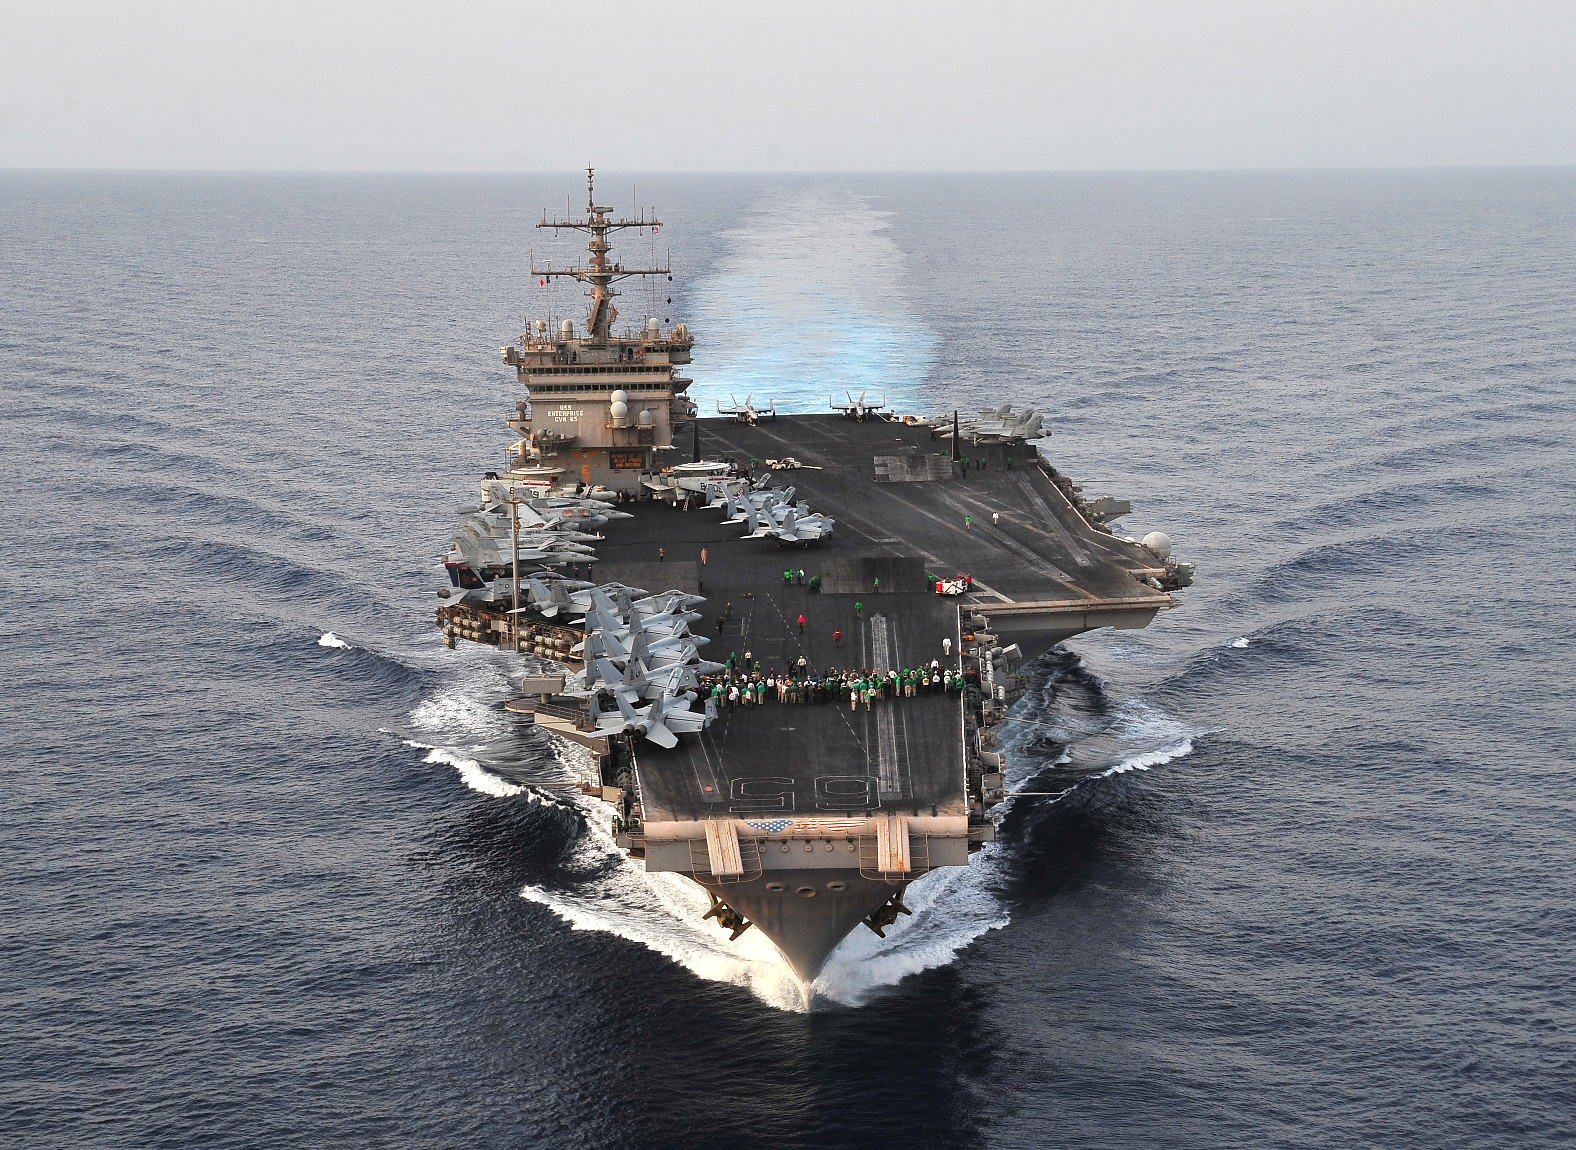
\includegraphics[width=0.495\textwidth]{Images/Public_domain/US_Navy_110607-N-JL826-140_The_aircraft_carrier_USS_Enterprise_(CVN_65)_transits_the_Gulf_of_Aden_while_conducting_maritime_security_operations_in_}}
    \subcaptionbox{\label{fig:aircraft_carrier_landing_backwash}} {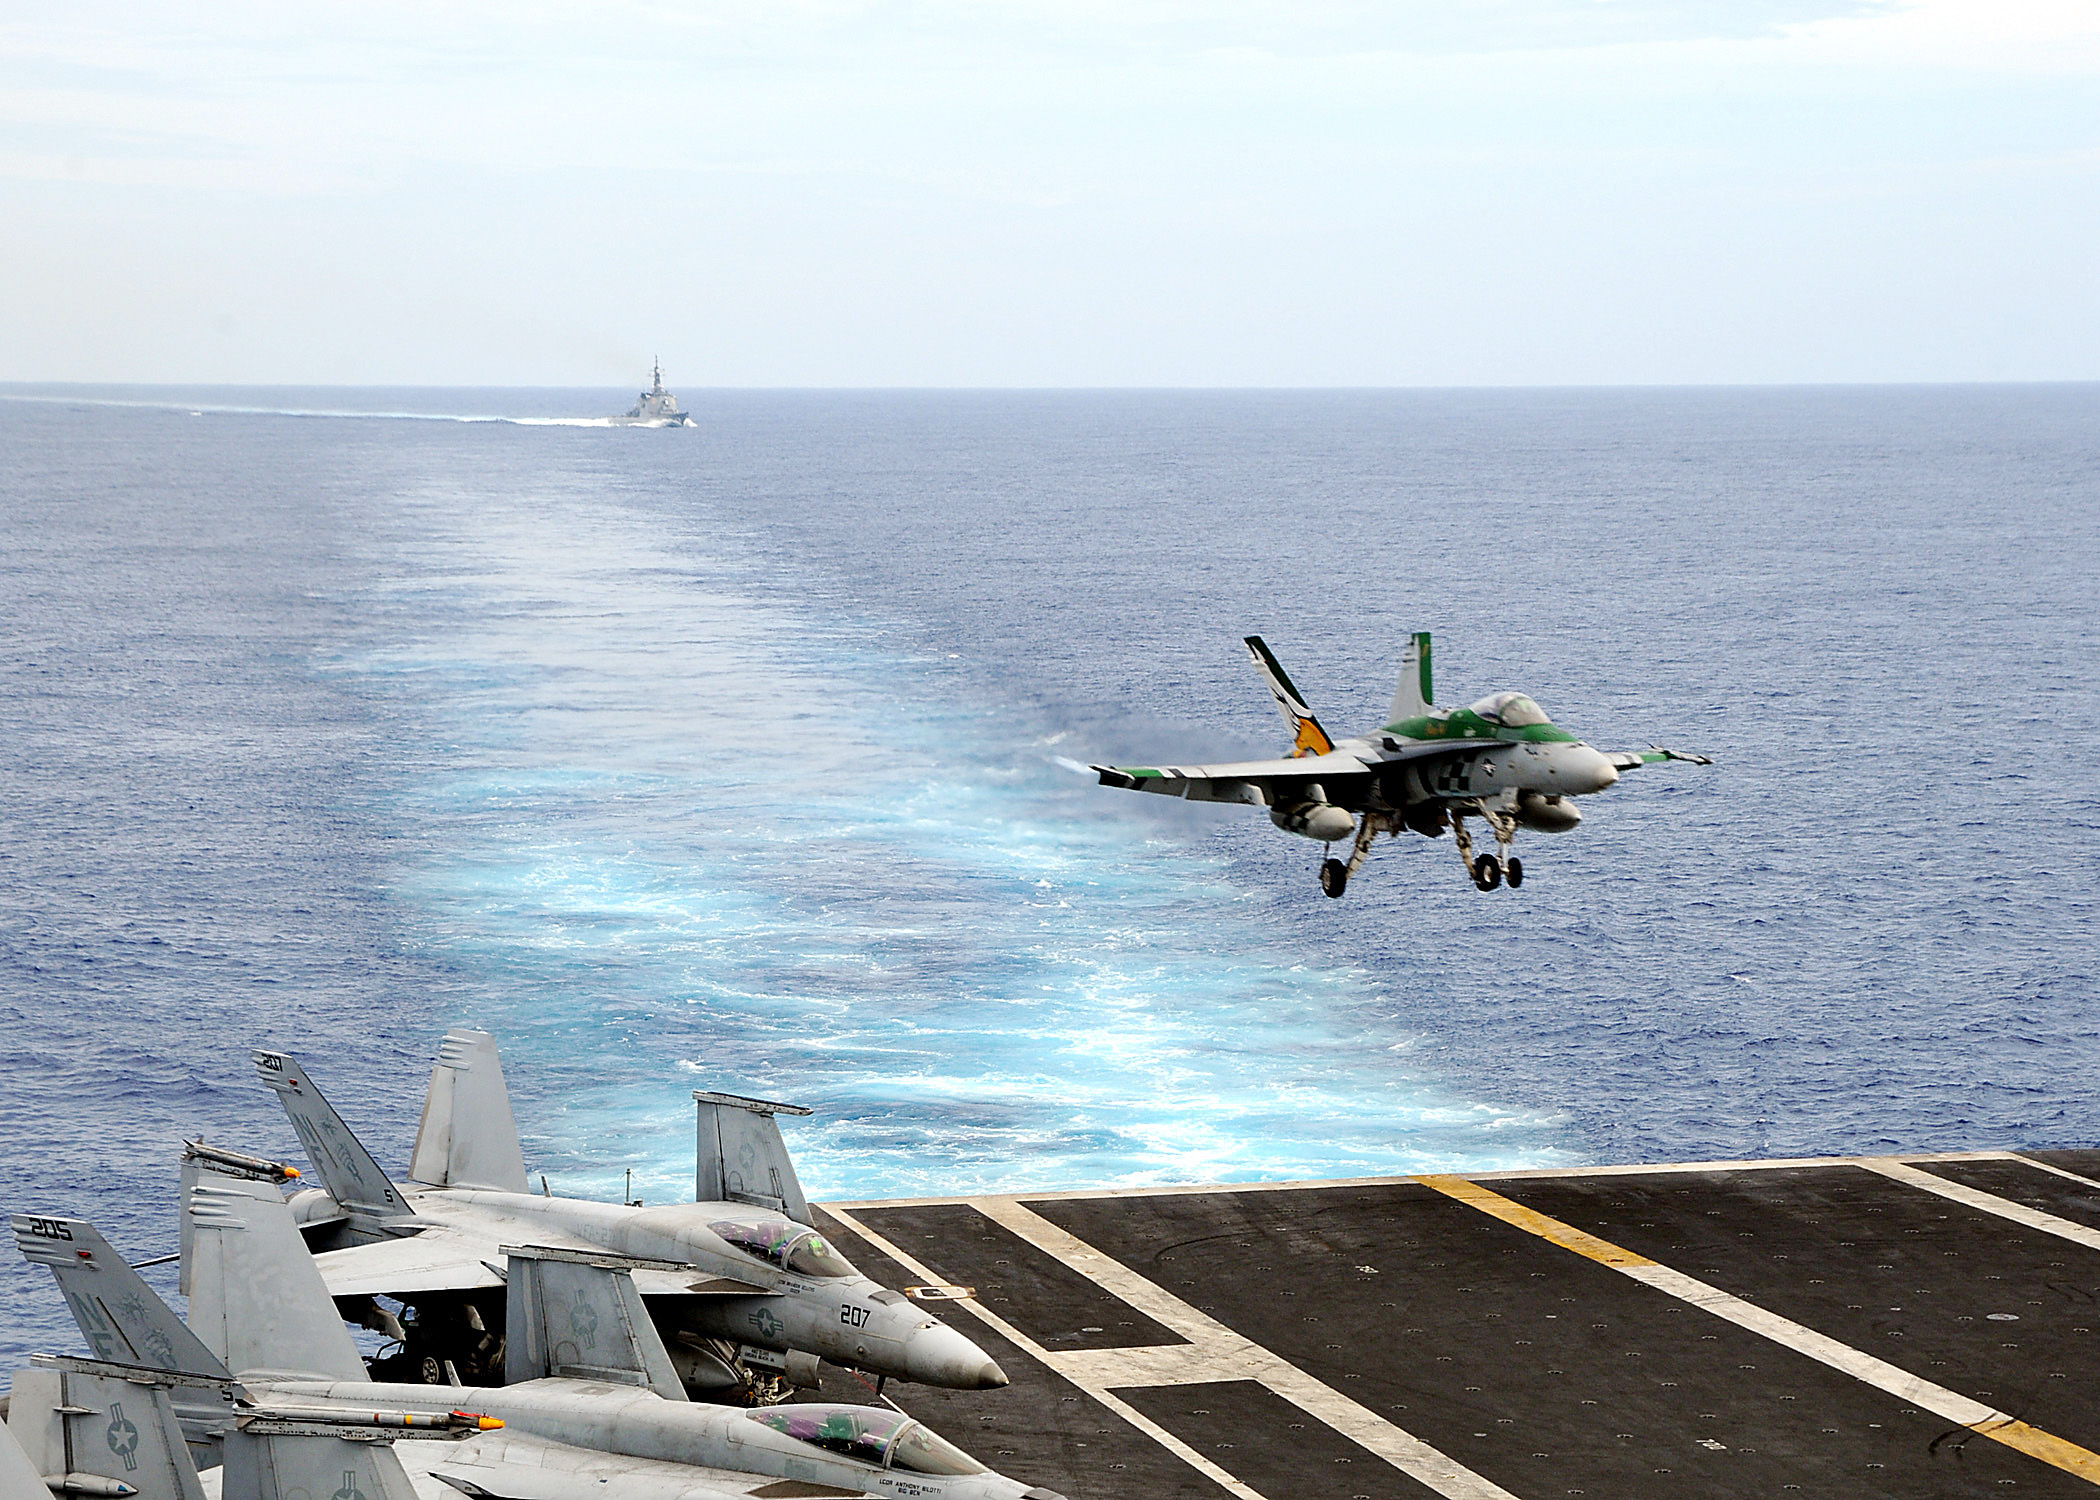
\includegraphics[width=0.495\textwidth]{Images/Public_domain/US_Navy_091113-N-6567V-068_F-A-18C_Hornet_lands_on_the_aircraft_carrier_USS_George_Washington_(CVN_73)}}
    \caption{Aircraft carriers. Note the backwash created behind the ships, serving as a reference for aircraft pilots during landing. \subrefp{fig:aircraft_carrier_full_wake} The aircraft carrier USS Enterprise (CVN 65). \subrefp{fig:aircraft_carrier_landing_backwash} An F/A-18 Hornet landing on an aircraft carrier.}
    \label{fig:aircraft_carriers_and_backwash}
\end{figure}

%TODO: Replace URL with reference
In a real situation the pilot can look at the backwash created by the carrier in order to find the right angle to approach the carrier with, as clearly can clearly be seen in \figref{fig:aircraft_carrier_landing_backwash} and in \citep{alivewithpassion2007}. In a simulation, it is important that the pilot has the same possibility. It is therefore necessary that ships leave a wake in the simulation that looks and behaves as a real wake and that consists of both waves created by the ship and of water behind the ship containing a lot of air, making it significantly brighter than the rest of the water. It is valuable if this wake keeps alive and looks as a real wake for as long time as possible, making it possible to determine the direction to a ship from a long distance even if only a single \idxs{wake}{line} is spoted.